\documentclass[usepdftitle=false]{beamer}

\usepackage[utf8]{inputenc}
\usetheme{Singapore}
\usepackage{xcolor}
\setbeamertemplate{footline}[frame number]
% \setbeamercovered{transparent}
%\usecolortheme{crane}

\title[IFT3515]{IFT 3515\\Fonctions à plusieurs variables\\Optimisation sans contraintes\\Méthode de Newton}
\author[Fabian Bastin]{Fabian Bastin\\DIRO\\Université de Montréal}
%\date{Hiver 2017}
\date{}


\usepackage{enumerate}
\usepackage[francais]{babel}

\usepackage{easybmat}
\usepackage{graphicx}

\newtheorem{defn}{Définition}
\newtheorem{lem}{Lemme}
\newtheorem{thm}{Théorème}
\newtheorem{coro}{Corollaire}

\def\red{\color{red}}
\def\blue{\color{blue}}

\def\co{\mathcal{o}}

\def\cB{\mathcal{B}}
\def\cR{\mathcal{R}}

\def\bu{\boldsymbol{u}}

\begin{document}
\frame{\titlepage}

% ------------------------------------------------------------------------------------------------------------------------------------------------------

\begin{frame}
\frametitle{Directions de descente plus générales}

Soit $B_k$ une matrice symétrique, définie positive, et définissons la direction de recherche $d_k$ comme la solution du système linéaire
$$
B_k d_k = - \nabla f(x_k)
$$

\mbox{}

$d_k$ est une direction de descente puisque
$$
- \nabla f(x_k)^T B_k^{-1} \nabla f(x_k) < 0.
$$

\mbox{}

$d_k$ est solution du problème
$$
\min_{d \in \cR^n} m(x_k + d) = f(x_k) + \nabla f(x_k)^T d + \frac{1}{2} d^T B_k d.
$$

\end{frame}

\begin{frame}
\frametitle{Remarques}

$d_k$ correspond à la direction de plus forte pente si la norme
$$
\| x \|^2_{B_k} = x^T B_k x,\ x \in \cR^n
$$
est utilisée au lieu de la norme euclidienne (norme 2).
Ce changement de métrique peut être vu comme une technique de préconditionnement utilisée pour accélérer la méthode de plus forte pente.

\mbox{}

Si la matrice hessienne $H_k = \nabla^2 f(x_k)$ est définie positive, et $B_k = H_k$, il s'agit de la méthode de Newton.

\mbox{}

Si $B_k$ change à chaque itéré $x_k$, une méthode basée sur la direction de recherche $d_k$ est appele {\blue méthode à métrique variable}.
En particulier, la méthode de Newton est une méthode à métrique variable.

\end{frame}

\begin{frame}
\frametitle{Méthode de Newton}

Nous supposons que $f \in C^2$.
La méthode de Newton pour des fonctions multivariées est une extension directe de la méthode pour les fonctions à une seule variable.

\mbox{}

Considérons le développement de Taylor au deuxième ordre autour de $x_k$:
\begin{align*}
f(x) = & f(x_k) + \nabla f(x_k)^T(x-x_k) + \frac{1}{2} (x-x_k)^T \nabla^2 f(x_k) (x-x_k) \\
& + o(\| x - x_k \|^2)
\end{align*}
et construisons le modèle quadratique
$$
m(x) = f(x_k) + g_k^T(x-x_k) + \frac{1}{2} (x-x_k)^T H_k (x-x_k)
$$
où $g_k = \nabla f(x_k)$ et $H_k = \nabla^2 f(x_k)$.

\end{frame}

\begin{frame}
\frametitle{Méthode de Newton}

Soit $s_k = x-x_k$. Le modèle peut se réécrire comme
$$
m(s_k) = f(x_k) + g_k^T s_k + \frac{1}{2} s_k^T H_k s_k
$$
Si $H_k$ est définie-positive, $m(s_k)$ est strictement convexe, et son minimum s'obtient en annulant la dérivée de $m(s_k)$ par rapport à $s_k$, soit
$$
0 = g_k + H_k s_k
$$
conduisant à
$$
s_k = -H_k^{-1}g_k
$$
Note: nous ne calculons pas $H_k^{-1}$ pour des questions de précision numériques, mais nous obtenons $s_k$ en résolvant le système linéaire
$$
H_k s_k = -g_k
$$

\end{frame}

\begin{frame}
\frametitle{Méthode de Newton: difficultés}

Comme dans le cas univarié, la convergence n'est assurée que si le point de départ est suffisamment proche de la solution, et est alors quadratique.

\mbox{}

On peut obtenir la convergence globale en utilisant la direction de Newton comme direction de descente avec une méthode de recherche linéaire, en s'assurant que $\alpha_k$ puisse prendre la valeur 1 afin d'assurer une convergence quadratique au cours des dernières itérations.

\end{frame}

\begin{frame}
\frametitle{Fonctions non convexes}

Que faire si la matrice hessienne n'est pas définie positive? Dans ce cas, le modèle n'est pas convexe, et annuler le gradient, pour autant qu'on puisse le faire, ne garantit pas de trouver un minimum local.

\mbox{}

On ajouter un multiple $\nu > 0$ de la matrice identité pour ``corriger'' la courbure de la fonction. En effet, considérons une matrice carrée $A$ ayant une valeur propre $\lambda$ associée au vecteur propre $u$:
$$
A u = \lambda u
$$
Dans ce cas,
$$
(A+\nu I)u = Au+\nu u = \lambda u + \nu u = (\lambda + \nu) u
$$
Autrement, $A+\nu I$ est à présent associée à la valeur propre $\lambda + \nu$.

\end{frame}

\begin{frame}
\frametitle{Fonctions non convexes}

Le spectre d'une matrice $A$ carrée est l'ensemble de ses valeurs propres $\lbrace \lambda_1,\dots,\lambda_s \rbrace$, en supposant que nous avons $s$ valeurs propres distinctes.
Du raisonnement précédent, le spectre de $A+\nu I$ est $\lbrace \lambda_1+\nu,\dots,\lambda_s + \nu \rbrace$ et donc $A + \nu I$ est définie positive si $\nu > \lambda_{\min}$.

\mbox{}

Soit $\nu$ tel que $H_k + \nu I$ est définie positive. De ce qui précède, $-(H_k + \nu I)^{-1} \nabla f(x_k)$ est une direction de descente et nous pouvons appliquer la méthode de recherche linéaire avec backtracking.

\mbox{}

Supposons que la sous-séquence d'itérés $\lbrace x_{k_j} \rbrace$ converge vers $x^*$, et que la condition suffisante d'optimalité au deuxième ordre est satisfaite en $x^*$, i.e. $\nabla f(x^*) = 0$ et $\nabla^2 f(x^*)$ est définie positive.
Si $f \in C^2$, $\nabla^2 f(x)$ est définie positive dans un voisinage de $x^*$ et $\nu = 0$ pour $j$ assez grand, de sorte que la méthode se réduit à la recherche linéaire de Newton.

\end{frame}

\begin{frame}
\frametitle{Méthodes quasi-Newton}

Le calcul de la matrice hessienne peut être coûteux, surtout en grande dimension.

\mbox{}

Considérons à nouveau le modèle quadratique
$$
m_k(x) = f(x_k) + g_k^T(x-x_k) + \frac{1}{2} (x-x_k)^T H_k (x-x_k)
$$
où $g_k = \nabla f(x_k)$, mais cette fois, $H_k$ est pris comme approximation de $\nabla^2 f(x_k)$.

\mbox{}

On parle alors de méthode {\red quasi-Newton}.

\mbox{}

On va s'inspirer de la méthode de la sécante pour les fonctions univariées.

\end{frame}

\begin{frame}
\frametitle{Condition de la sécante}

Comme de le cas univarié, nous exigerons que
$$
\nabla m_{k+1}(x_k) = \nabla f(x_k),\ 
\nabla m_{k+1}(x_{k+1}) = \nabla f(x_{k+1})
$$
La deuxième inégalité suit directement de la définition du modèle, mais il va falloir imposer une technique pour préserver la première.
En particulier,
$$
\nabla m_{k+1}(x_{k+1}) - \nabla m_{k+1}(x_k) = \nabla f(x_{k+1}) - \nabla f(x_k)
$$
Comme
$$
\nabla m_{k+1}(x) = g_{k+1} + H_{k+1}(x-x_{k+1}),
$$
nous avons
$$
\nabla m_{k+1}(x_{k+1}) - \nabla m_{k+1}(x_k) = H_{k+1}(x_{k+1} - x_k)
$$
La {\red condition de la sécante} peut dès lors s'énoncer comme
$$
H_{k+1}(x_{k+1} - x_k) = \nabla f(x_{k+1}) - \nabla f(x_k)
$$

\end{frame}

\begin{frame}
\frametitle{Condition de la sécante}

En supposant que $H_{k+1}$ est inversible, la condition peut se réécrire comme
$$
s_k = H_{k+1}^{-1}y_k
$$
où $s_k = x_{k+1} - x_k$ et $y_k = \nabla f(x_{k+1}) - \nabla f(x_k)$.

\mbox{}

De nombreuses matrices répondent à ces conditions, et il faudra imposer des conditions supplémentaires.

\mbox{}

Comme la matrice hessienne d'une fonction de classe $C^2$ est symétrique, nous exigerons en particulier que $H_{k+1}$ soit symétrique.

\end{frame}

\begin{frame}
\frametitle{BFGS}

Nous imposerons de plus que l'approximation ne change pas trop d'un itéré à l'autre en considérant le programme
\begin{align*}
\min_H & \| H^{-1} - H^{-1}_k \|_F \\
\mbox{tel que } & s_k = H^{-1}y_k \\
& H = H^T
\end{align*}
où $\| \cdot \|_F$ est la norme de Frobenius.
La norme de Frobenius d'une matrice $A \in \cR^{m \times n}$ est
$$
\| A \|_F = \sqrt{\sum_{i=1}^m \sum_{i=1}^n | a_{ij} |^2 }
$$
Cela conduit à l'approximation la plus populaire en optimisation, du nom de BFGS (Broyden-Fletcher-Goldfarb-Shanno), et nous la noterons $B_k$ au lieu de $H_k$.

\end{frame}

\begin{frame}
\frametitle{BFGS}
	
\begin{center}
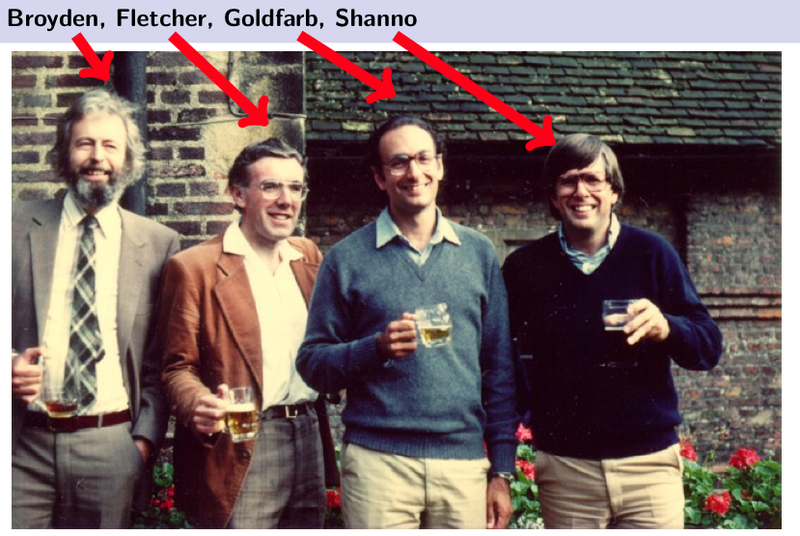
\includegraphics[width=0.9\textwidth]{bfgs.png}
\end{center}
{\footnotesize{Source: \url{http://aria42.com/blog/2014/12/understanding-lbfgs}}}
	
\end{frame}

\begin{frame}
\frametitle{BFGS}

Les détails sont techniques, et sont laissés sous silence\ldots

\mbox{}

{\red Mise à jour BFGS}

$$
B_{k+1} = B_k - \frac{B_k s_k s_k^T B_k}{s_k^T B_k s_k} + \frac{y_k y_k^T}{y_k^T s_k}
$$

{\red Mise à jour de l'inverse}

$$
B_{k+1}^{-1} = \left( I - \frac{s_k y_k^T}{s_k^T y_k} \right) B_k^{-1}  \left( I - \frac{y_k s_k^T}{y_k^T s_k} \right) + \frac{s_k s_k^T}{y_k^T s_k}
$$

\mbox{}

Par abus de langage, on parle souvent de l'approche BFGS pour désigner la recherche linéaire utilisant l'approximation BFGS.
	
\end{frame}

\begin{frame}
\frametitle{Notes}

La condition de la sécante s'écrit
$$
B_{k+1} s_k = y_k
$$
de sorte que
$$
s_k^T y_k = s_k^T B_{k+1} s_k > 0
$$
si $B_{k+1}$ est définie positive.

\mbox{}

En d'autres mots, vouloir que $B_{k+1}$ soit définie positive nous impose $s_k^T y_k > 0$.

\mbox{}

Supposons que nous travaillons avec une recherche linéaire par backtracking et que la condition de courbure dans les conditions de Wolfe tienne, i.e.
$\nabla f(x_k + \alpha_k d_k )^T d_k \geq \beta_2 \nabla f(x_k)^T d_k$ avec $\beta_2 < 1$. Alors, comme $d_k$ est une direction de descente,
\begin{align*}
s_k^T y_k = \alpha_k d_k^T y_k &= \alpha_k (\nabla f(x_k+\alpha_k d_k)-\nabla f(x_k))^T d_k \\
& \geq \alpha_k(\beta_2-1)\nabla f(x_k)^T d_k > 0.
\end{align*}

\end{frame}

\begin{frame}
\frametitle{Notes}

Supposons que $B_k$ est définie positive. Alors, $B_k^{-1}$ est elle-même définie positive, et $\forall x \ne 0$,
\begin{align*}
x^T B_{k+1}^{-1} x &=
x^T \left(
\left( I - \frac{s_k y_k^T}{s_k^T y_k} \right) B_k^{-1}  \left( I - \frac{y_k s_k^T}{y_k^T s_k} \right) + \frac{s_k s_k^T}{y_k^T s_k}
\right) x \\
&=
\left( x^T - \frac{x^Ts_k}{s_k^T y_k} y_k^T \right) B_k^{-1}  \left( x - \frac{s_k^Tx}{y_k^T s_k}y_k  \right) + \frac{x^Ts_k s_k^Tx}{y_k^T s_k} \\
& \geq 0
\end{align*}
Si $x^Ts_k \ne 0$, $x^T B_{k+1}^{-1} x > 0$ et $B_{k+1}^{-1}$ est définie positive, de même que $B_{k+1}$.
Supposons que $x^Ts_k = 0$. Alors
$$
x^T B_{k+1}^{-1} x = x^T B_k^{-1}x > 0
$$

\mbox{}

En d'autres termes, la mise à jour BFGS maintient le caractère défini positif.
	
\end{frame}

\begin{frame}
\frametitle{Initialisation de la mise-à-jour BFGS}

Le choix de $B_0$ affecte la convergence de la méthode.
Quelques possibilités sont
\begin{itemize}
\item
une approximation numérique, par différence finie ou centrale, de la matrice hessienne (coûteux: $O(n^2)$)
\item
$B_0 = I$, la matrice identité.
\item
$B_0 = diag(h_1,h_2,\ldots,h_n)$, où $h$ capture l'échelle des variables (si connu).
\end{itemize}

\end{frame}

\begin{frame}
\frametitle{Recherche linéaire quasi-Newton}

\begin{thm}[théorème 3.6, Nocedal \& Wright]
Supposons que $f: \cR^n \rightarrow \cR$ est deux fois continûment différentiable.
Considération l'itération
$$
x_{k+1} = x_k + \alpha_k d_k
$$
où $\alpha_k$ satisfait les conditions de Wolfe avec $\beta_1 \leq \frac{1}{2}$.
Si la séquence $\{ x_k \}$ converge vers un point $x^*$ tel que $\nabla f(x^*) = 0$ et $\nabla^2 f(x^*)$
est definie positive, et si la direction de recherche satisfait
$$
\lim_{k \rightarrow \infty} \frac{\|\nabla f(x_k) + \nabla^2 f(x_k) d_k \|}{\|d_k\|} = 0
$$
alors
\begin{enumerate}
\item 
$\alpha_k = 1$ est admissible pour tout $k$ plus grand qu'un certain $k_0$,
\item
si $\alpha_k = 1$ pour tout $k > k_0$, $\{ x_k \}$ converge vers $x^*$ superlinéairement.
\end{enumerate}
\end{thm}

\end{frame}

\end{document}